\documentclass[tikz,border=5pt,png]{standalone}
\usepackage{tikz}
\usetikzlibrary{shapes,backgrounds,calc,positioning}
\usepackage[utf8]{inputenc}
\usepackage[T1]{fontenc}
\renewcommand{\familydefault}{\sfdefault}

\begin{document}

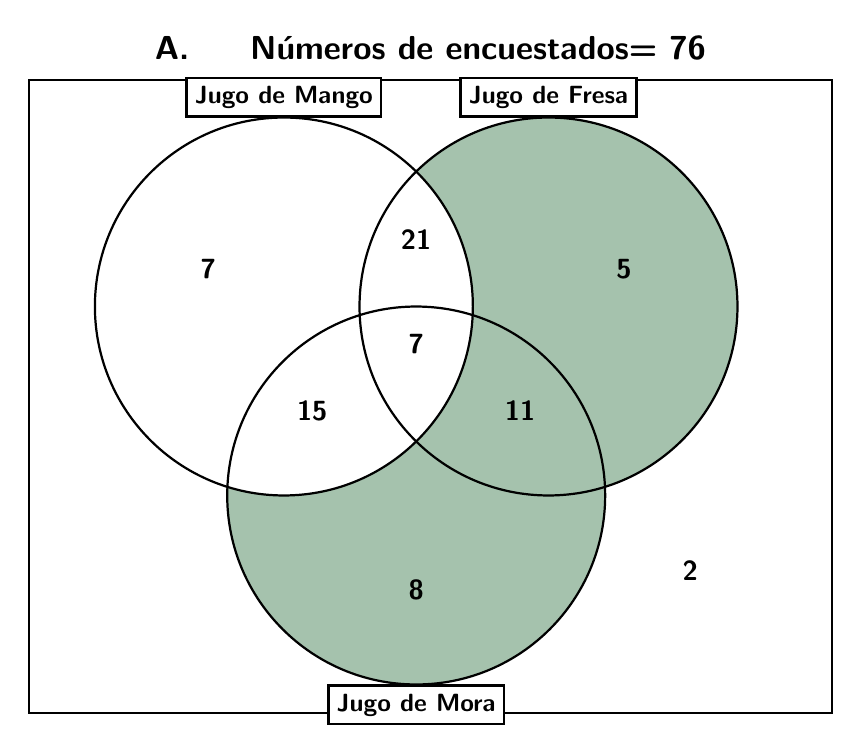
\begin{tikzpicture}[thick, scale=1.2]
  % Definición de colores
  \definecolor{shadedregion}{RGB}{165, 194, 173} % Verde grisáceo de la imagen
  \definecolor{labelbox}{RGB}{255, 255, 255} % Blanco para etiquetas

  % Coordenadas de los centros y radio
  \coordinate (M) at (-0.8, 0.8); % Mango (Arriba Izquierda)
  \coordinate (F) at (2.0, 0.8);  % Fresa (Arriba Derecha)
  \coordinate (Mo) at (0.6, -1.2); % Mora (Abajo)
  \def\R{2.0} % Radio de los círculos

  % --- Sombreado Correcto para la Imagen A ---
  % La región sombreada es (Fresa U Mora) - Mango.
  % Usamos un enfoque de capas para lograr esto.

  % 1. Primero, rellenamos los círculos de Fresa y Mora con el color de sombreado.
  % Esto crea la unión de Fresa y Mora.
  \fill[shadedregion] (F) circle (\R);
  \fill[shadedregion] (Mo) circle (\R);

  % 2. Luego, rellenamos el círculo de Mango con BLANCO.
  % Al hacerlo encima, "borramos" las partes de Fresa y Mora que se superponen con Mango.
  \fill[white] (M) circle (\R);

  % --- Contornos de los Círculos ---
  % Dibujamos los contornos al final para que queden nítidos sobre el sombreado.
  \draw (M) circle (\R);
  \draw (F) circle (\R);
  \draw (Mo) circle (\R);

  % --- Conjunto Universal (Marco) y Título ---
  \draw (-3.5, -3.5) rectangle (5.0, 3.2);
  \node[anchor=south, font=\bfseries\large, align=center] at (0.75, 3.3) {A. \hspace{1em} Números de encuestados= 76};

  % --- Etiquetas de los Conjuntos ---
  \tikzset{setlabel/.style={draw, fill=labelbox, font=\bfseries\small, inner sep=3pt}}
  \node[setlabel, anchor=south] at ($(M) + (0, \R)$) {Jugo de Mango};
  \node[setlabel, anchor=south] at ($(F) + (0, \R)$) {Jugo de Fresa};
  \node[setlabel, anchor=north] at ($(Mo) - (0, \R)$) {Jugo de Mora};

  % --- Números (Datos) ---
  % Colocación de los números en sus regiones respectivas.
  \node[font=\bfseries] at (-1.6, 1.2) {7};  % Solo Mango
  \node[font=\bfseries] at (2.8, 1.2) {5};   % Solo Fresa (Sombreado)
  \node[font=\bfseries] at (0.6, -2.2) {8};  % Solo Mora (Sombreado)
  \node[font=\bfseries] at (0.6, 1.5) {21};  % Mango y Fresa
  \node[font=\bfseries] at (-0.5, -0.3) {15}; % Mango y Mora
  \node[font=\bfseries] at (1.7, -0.3) {11};  % Fresa y Mora (Sombreado)
  \node[font=\bfseries] at (0.6, 0.4) {7};   % Los tres
  \node[font=\bfseries] at (3.5, -2.0) {2};   % Fuera

\end{tikzpicture}

\end{document}